\documentclass[12pt, letterpaper, titlepage]{article}

\usepackage{amsmath}
\usepackage{amssymb}
\usepackage{booktabs}
\usepackage{amsthm}
\usepackage{graphicx}
\usepackage[margin=1in]{geometry}
\usepackage{hyperref, url}
\hypersetup{colorlinks = true, linkcolor = blue, citecolor=blue, urlcolor =
  blue}
\usepackage{natbib}
\usepackage{enumitem}
\usepackage{setspace}

\usepackage[pagewise]{lineno}
%\linenumbers*[1]
% %% patches to make lineno work better with amsmath
\newcommand*\patchAmsMathEnvironmentForLineno[1]{%
 \expandafter\let\csname old#1\expandafter\endcsname\csname #1\endcsname
 \expandafter\let\csname oldend#1\expandafter\endcsname\csname end#1\endcsname
 \renewenvironment{#1}%
 {\linenomath\csname old#1\endcsname}%
 {\csname oldend#1\endcsname\endlinenomath}}%
\newcommand*\patchBothAmsMathEnvironmentsForLineno[1]{%
 \patchAmsMathEnvironmentForLineno{#1}%
 \patchAmsMathEnvironmentForLineno{#1*}}%

\AtBeginDocument{%
 \patchBothAmsMathEnvironmentsForLineno{equation}%
 \patchBothAmsMathEnvironmentsForLineno{align}%
 \patchBothAmsMathEnvironmentsForLineno{flalign}%
 \patchBothAmsMathEnvironmentsForLineno{alignat}%
 \patchBothAmsMathEnvironmentsForLineno{gather}%
 \patchBothAmsMathEnvironmentsForLineno{multline}%
}

% control floats
\renewcommand\floatpagefraction{.9}
\renewcommand\topfraction{.9}
\renewcommand\bottomfraction{.9}
\renewcommand\textfraction{.1}
\setcounter{totalnumber}{50}
\setcounter{topnumber}{50}
\setcounter{bottomnumber}{50}

\newcommand{\jy}[1]{\textcolor{blue}{JY: #1}}
\newcommand{\eds}[1]{\textcolor{red}{EDS: (#1)}}
\newcommand{\mc}[1]{\textcolor{green}{MC: (#1)}}


\title{On Sample Size for Block Bootstrap Confidence Intervals 
  to Have Desired Coverage Rates}


\author{Mathew Chandy, Elizabeth Schifano,
%   \href{mailto:mathew.chandy@uconn.edu}
% {\nolinkurl{mathew.chandy@uconn.edu}}\\
  and Jun Yan\\[1ex]
  Department of Statistics, University of Connecticut\\
}
\date{}


\begin{document} 
\maketitle


\begin{abstract}
Block bootstrap is widely used in constructing confidence intervals for
parameters estimated from stationary time series. Theoretically, the method
should provide valid confidence intervals as the length of the time series goes
to infinity. In practice, however, it is necessary to know how large of a
finite sample is required for block bootstrap confidence intervals to work
well. This study aims to answer this question in a simple simulation setting
where the data are generated from a first-order autoregressive process. The
empirical coverage rates of several commonly used bootstrap confidence
intervals for the mean, standard deviation, and the lag-1 autocorrelation
coefficient are compared. A quite large sample is found necessary for the
intervals to have the right coverage rates even when estimating a simple
parameter like the mean. Some block bootstrap methods could fail when
estimating the lag-1 autocorrelation. It is surprising that the coverage
property even deteriorates as the sample size increases with some commonly
used block bootstrap confidence intervals including the percentile intervals
and Bias-Corrected intervals.


\bigskip
\noindent{\sc Keywords}:
dependent data; resampling; simulation; time series
\end{abstract}


\doublespace


\section{Introduction}
\label{sec:intro}


Block bootstrap is a tool to construct confidence intervals (CI) to make
inferences about dependent data. Essentially, it depends on correct estimation
of the uncertainty in the estimation. Early ideas were developed by
\citet{hall1985resampling, carlstein1986use,kunsch1989jackknife}. It has since
been applied in various fields, for instance, econometrics
\citep{mackinnon2006bootstrap} and meteorology \citep{varga2017generalised}.
Block bootstrap is especially useful for serially dependent data when the
serial dependence is not specified or not of primary interest. The method is
expected to produce CIs with coverage rates matching their nominal levels as
the sample size grows. However, when dealing with finite sample sizes, an
important question is how large the sample size must be for block bootstrap
CIs to have the desired coverage rates.


For independent data, extensive research has explored the effectiveness of
bootstrap standard errors in providing accurate uncertainty measures. For
example, \citet{hesterberg2015teachers} observes that while percentile-based
CIs for the mean parameter are more accurate than $t$-intervals for larger
sample sizes, they accuracy diminishes for smaller sample sizes. The optimal
parameter estimation of a distribution, according to
\citet{chernick2009revisiting}, depends on the sample size, the number of
bootstrap replicates, and the confidence level. In structural equation
modeling, \citet{nevitt2001performance} find that a sample size of 200--1000
is sufficient for interval estimation using standard nonparametric bootstrap.
Estimating variance component, \citet{burch2012nonparametric} report that as
the sample size increases under a normal distribution, nonparametric bootstrap
methods approach the coverage of a pivotal quantity as the sample size, but
for other distributions, the coverage can deteriorate. In estimating the
correlation coefficient of bivariate normal data, \citet{puth2015variety} note
that even for a sample size of~$100$ with true correlation coefficient~0,
bootstrap methods are less accurate than the Fisher's transformation. The
prevailing consensus highlights the necessity of a substantial sample size for
bootstrap CIs to attain the desired coverage.


Limited research has offered practical guidance concerning the requisite sample
size for employing block bootstrap inference with dependent data. In the
context of linear regression involving dependent data, where regression errors
stem from a homoscedastic autoregressive process of order-1, the investigation
conducted by \citet{goncalves2005bootstrap} reveals that, in cases of small
sample sizes, standard error estimates derived from the moving block bootstrap
approach may demonstrate greater accuracy than those based on closed-form
asymptotic estimates. Nonetheless, even when considering a substantial sample
size of ~$1024$, confidence intervals generated through the moving block
bootstrap method still fail to adequately encompass the target parameter. The
scarcity of existing literature addressing the necessary sample sizes
conducive to the efficacy of block bootstrap techniques has spurred the
initiation of the present study.


The goal of this paper is to provide recommendations on necessary sample size
for block bootstrap with dependent data, similar to what was done for basic
bootstrap in \citet{hesterberg2015teachers}. We consider a simple situation of
a stationary time series, where the parameters of interests are the mean,
standard deviation, and the first-order autocorrelation coefficient. We
compare six variants of block bootstrap CIs from the literature
\citep{diciccio1996bootstrap, rice2006mathematical}: a standard normal CI, and
a Student's $t$ CI, a percentile CI, a bias-corrected CI, a bias-corrected and
accelerated ($BC_a$) CI, and a recentered percentile CI proposed in this article.
Their empirical
coverage rates at different sample sizes and dependence levels are compared in
a simulation study. The results of this study suggest that recovery of
temporal dependence parameters is reliant on the type of interval used.


The remainder of the paper is organized as follows. Section~\ref{sec:bbci}
reviews block bootstrap procedures and how to use block bootstrap estimates to
construct CIs; a simple CI obtained by recentering at the point estimate is
proposed for comparison. Section~\ref{sec:simu} reports a simulation study
comparing the coverage rates of six block bootstrap CIs. A discussion
concludes in Section~\ref{sec:disc}.


\section{Block Bootstrap CIs}
\label{sec:bbci}


Consider a stationary time series $\{X_t: t = 1, \ldots, n\}$ with length~$n$.
Our goal is to construct a CI for a parameter $\theta$ in the data generating
model of the series. Suppose that $\hat\theta_n$ is a point estimator
of~$\theta$ based on the observed series. Bootstrap is a powerful approach to
construct CIs. If the observations in the series were independent, a standard
nonparametric bootstrap procedure would draw a large number~$B$ bootstrap
copies of the observed data, and calculate an estimate $\hat\theta_n^{(b)}$
for each copy $b = 1, \ldots, B$. The uncertainty of $\hat\theta_n$ is then
estimated by the empirical uncertainty of the $\hat\theta_n^{(b)}$'s. When
serial dependence is present, the bootstrap procedure needs to preserve the
serial dependence. Block bootstrap was motivated for this situation. 


\subsection{Block Bootstrap}


Block bootstrap preserves the serial dependence in the observed data by
partitioning the data into blocks and performing bootstrap on the blocks. In
particular, consider block size~$l$ and, for convenience, suppose that $n$ is
a multiple of $l$ such that there are $k = n / l$ blocks. Each block~$j$ is
$Y_j = \{X_{(j - 1) l + 1}, \ldots, X_{(j - 1) l + l}\}$, $j = 1, \ldots, k$.
Then, we sample $k$ blocks of $Y_j$'s from the set $\{Y_1, \ldots, Y_k\}$ with
replacement and concatenate the $k$ sampled blocks in the order they are
picked to form a bootstrap sample of the data. The formation of the bootstrap
sample ensures that the between-block dependence is weak and that the
within-block serial dependence is preserved. Because the blocks here are
non-overlapping, this bootstrap approach is known as non-overlapping block
bootstrap, or simple block bootstrap.


Alternatively, block-bootstrap can be done with overlapping or moving blocks.
Define moving blocks $Z_j = \{X_j, \ldots, X_{j + l - 1}\}$,
$j = 1, \ldots, n - l + 1$. Now we draw $k$ blocks from the $(n - l + 1)$
blocks of $Z_j$'s with replacement and then align them in the order they were
picked to form a block bootstrap sample. If $n$ is not a multiple of~$l$, the
last block selected will be reduced in size so that the final size of the
block bootstrap sample is $n$. It is also possible to implement moving block
bootstrap while allowing blocks to wrap around the end of the series. In other
words, define moving blocks (assuming $l > 1$) as:
\begin{equation}
Z_j =
    \begin{cases}
        \{X_j, \ldots, X_{j + l - 1}\}, & \text{if } j = 1, \dots, n - l + 1,\\
        \{X_j, \ldots, X_n, X_1, \ldots, X_{j-n+l-1}\}, & \text{if } j = n - l
        + 2 ,\dots, n.
    \end{cases}
\end{equation}
This version does not require that $n/l$ be an integer.


The block size~$l$ needs to be chosen with care. It should be large enough for
each bootstrap sample to preserve the serial dependence, yet small enough for
there to be a large number of blocks to give sufficient variability between
each bootstrap sample. As $n$ increases, both~$l$ and $n / l$ should also
increase. To achieve this, $l$ is often assigned a value as a function of $n$.
A common function that is considered optimal is $l = \lceil n^{1/3} \rceil$
\citep{buhlmann1999block}, which was adopted in this study.


\subsection{Bootstrap CIs}


Suppose that we have repeated the steps in the last subsection $B$ times, and
that for $b \in \{1, \ldots, B\}$, we have obtained an estimator
$\hat\theta_n^{(b)}$ based on the $b$th bootstrap sample using the same method
that was applied to $\{X_t: t = 1, \ldots, n\}$ to obtain $\hat\theta_n$. Now
the question is how to construct a CI for $\theta$ using the $B$ bootstrap
point estimates $\{\hat\theta_n^{(1)}, \ldots, \hat\theta_n^{(B)}\}$. We
consider six kinds of CIs.


\paragraph{Standard Normal CI}
Assuming that $\hat\theta_n$ is asymptotically normally distributed with
$\theta$ as the mean, we just need an estimate of the standard error to
construct an approximate CI \citep[p.168]{efron1993introduction}. Let
$\widehat{\text{SE}}$ be the empirical standard error of the block bootstrap
copies of $\hat\theta_n^{(b)}$, $b = 1, \ldots, B$. Let $z_{(\alpha)}$ be the
upper $\alpha$ quantile of the standard normal distribution. A
$(1 - \alpha)100\%$ standard normal CI is
\[
(\hat{\theta}_{n} - z_{(1-\alpha/2)}\widehat{\text{SE}}, \quad
\hat{\theta}_{n} - z_{(\alpha/2)}\widehat{\text{SE}}).
\]
This CI is centered by the point estimator $\hat\theta_n$ and is symmetric. The
Standard CI is a table-based bootstrap interval approach. Its validity relies
on whether the distribution of $\hat\theta_n$ is reasonably well approximated
by its asymptotic normal distribution and whether the bootstrap
$\widehat{\text{SE}}$ approximates the true standard error.


\paragraph{Student's $t$ CI}
The procedure for constructing a Student's $t$ CI based on standard bootstrap
is described in \citet[p.158]{efron1993introduction}. Let $t_{(\alpha, k)}$ be
the upper $\alpha$ quantile of a $t$ distribution with $k$ degrees of freedom.
With block bootstrapping, a $(1 - \alpha)100\%$ Student's $t$ CI is
\[
(\hat{\theta}_{n} - t_{(1-\alpha/2), k - 1}\hat{\text{SE}}, \quad
\hat{\theta}_{n} - t_{(\alpha/2), k -1}\hat{\text{SE}}),
\]
%\eds{define $t_{(.)}$ and check the signs}  \mc{addressed}
where $k$ is the number of blocks. This CI is centered by the point estimator
$\hat\theta_n$ and is symmetric. Like the standard normal interval, the
Student's $t$ CI is a table-based bootstrap interval approach. In this case,
its validity relies on whether the distribution of $\hat\theta_n$ is
reasonably well approximation by the $t_{k-1}$ distribution with an expected
value of $\theta$, and whether the bootstrap $\widehat{\text{SE}}$
approximates the true standard error.


\paragraph{Percentile CI}
The percentile CI was first suggested in \citet{efron1979bootstrap}.
Let $\hat\theta_{n, \alpha}^{(b)}$ be the empirical $100\alpha$th percentile of
$\{\hat\theta_n^{(1)}, \ldots, \hat\theta_n^{(B)}\}$. The $(1 - \alpha)100\%$
empirical percentile CI is
\[
(\hat\theta_{n, \alpha/2}^{(b)}, \quad \hat\theta_{n, 1 - \alpha/2}^{(b)}).
\]
This CI is not necessarily centered by the point estimator $\hat\theta_n$. As
will be shown in our simulation study, this approach works well for the
marginal mean and standard deviation of a serially dependent process, but its
coverage of the temporal dependence deteriorates as $n$ increases, which is
contrary to what one would expect.


\paragraph{Bias Corrected ($BC$) Bootstrap CI}
The procedure for constructing a Bias Corrected Bootstrap CI based on standard
bootstrap is described in \citet{carpenter2000bootstrap}. Let
$b = \Phi^{-1}\{\#\{\hat\theta_n^{(b)} < \hat{\theta}_n\} / B\}$ for
$b \in \{1, \ldots, B\}$. Define $\alpha_1 = \Phi(2b - z_{\alpha/2})$ and 
$\alpha_2 = \Phi(2b - z_{1 - \alpha/2})$. A $(1 - \alpha)100\%~BC$ CI is
\[
(\hat\theta_{n, \alpha_1}^{(b)}, \quad \hat\theta_{n, \alpha_2}^{(b)}).
\]


\paragraph{Bias Corrected and Accelerated ($BC_a$) Bootstrap CI}
The $BC_a$ CI was first suggested in \citet{efron1987better}. Let
$\hat{z}_0 = \Phi^{-1}\{\#\{\hat\theta_n^{(b)} < \hat{\theta}_n\} / B\}$ for
$b \in \{1, \ldots, B\}$. Let $Z_{(i)}$ be the original sample without the
$i$th block $z_i$ for $i \in \{1, \ldots, k\}$, let $\hat{\theta}_{(i)}$ be
the statistic of $Z_{(i)}$, and let
$\hat{\theta}_{(.)} = \sum_{i=1}^{k} \hat{\theta}_{(i)} / k$. 
Let 
\[
\hat{a} = \frac{\sum_{i=1}^{k} (\hat{\theta}_{(.)} -
  \hat{\theta}_{(i)})^3}{6\{\sum_{i=1}^{k} (\hat{\theta}_{(.)} -
  \hat{\theta}_{(i)})^2\}^{3/2}}.
\]
Define
\[
\alpha_1 = \Phi\left(z_0 + \frac{z_{0} +
  z_{\alpha/2}}{1 - \hat{a}(\hat{z}_{0} + z_{\alpha/2})}\right)
\text{ and }
\alpha_2 = \Phi\left(z_0 + \frac{z_{0} +
  z_{1 - \alpha/2}}{1 - \hat{a}(\hat{z}_{0} + z_{1 - \alpha/2})}\right).
\]
A $(1 - \alpha)100\%~BC_a$ CI is
\[
(\hat\theta_{n, \alpha_1}^{(b)}, \quad \hat\theta_{n, \alpha_2}^{(b)}).
\]
This CI is not necessarily centered by the point estimator $\hat\theta_n$. The
$BC_a$ method corrects for bias and skewness of the $B$ bootstrap point
estimates $\{\hat\theta_n^{(1)}, \ldots, \hat\theta_n^{(B)}\}$ by including
bias-correction and acceleration factors. The acceleration factor refers to
the rate of change of the standard error of $\hat\theta_n$ with respect to
$\theta$.


\paragraph{Recentered Percentile CI}
\jy{Can we come up with a good name for the proposed method? Other people may
 cite this.} \mc{bias-centered? i'm not sure}
\jy{How about ``recentered percentile''? It has the same length as the
  percentile approach but is centered at the point estimate.} \mc{replaced
  all instances of "proposed
  method" with "recentered"}

We propose a CI that is centered at the point estimator and uses the variation
in the bootstrap estimates to construct the error bound. This interval requires
the computation of $\bar\theta_n^{(b)}$, the mean of all bootstrap point
estimates, and $\widehat{\text{bias}} = \bar\theta_n^{(b)} - \hat\theta_n$. A
$(1 - \alpha)100\%$ CI is
\[
(\hat\theta_{n, \alpha/2}^{(b)} - \widehat{\text{bias}}, \quad
\hat\theta_{n, 1 - \alpha/2}^{(b)} - \widehat{\text{bias}}).
\]
This CI is centered around $\hat\theta_n$ and can also be rewritten
as 
\[
(\hat\theta_n + \hat\theta_{n, \alpha/2}^{(b)} - \bar\theta_n^{(b)}, \quad
\hat\theta_n + \hat\theta_{n, 1 - \alpha/2}^{(b)} - \bar\theta_n^{(b)}).
\]
It is not necessarily symmetric, as different critical values are used to compute
the lower and upper bounds. It has the same width as the Percentile CI.


\section{Simulation Study}
\label{sec:simu}

\subsection{Design}
We designed a simulation study to compare the performance of the different
block bootstrap CI methods. In particular, we generated time series $X_t$ from
a 1st order auto-regressive (AR(1)) process:
\[
X_t = \phi X_{t-1} + \epsilon_t,
\]
where $\phi$ is an auto-regressive coefficient, and $\epsilon_t$ is a series of
independent errors from a normal distribution with mean zero and variance
$\sigma_{\epsilon}^2$. The strength of the serial dependence is controlled by
$\phi$, which was set to five levels: $\{-0.4, -0.2, 0.0, 0.2, 0.4\}$. The
series $X_t$ has mean zero and variance
$\sigma_x^2 = (1 - \phi^2) \sigma_{\epsilon}^2$, so for each value of $\phi$,
we set $\sigma_{\epsilon}^2 = 1 / (1 - \phi^2)$ such that $\sigma_x^2 = 1$.


Three target parameters of $X_t$ were considered:
1) $\mu = 0$, the mean of $X_t$;
2) $\sigma_x = 1$, the standard deviation of $X_t$; and
3) $\phi$, the lag-1 auto-correlation coefficient.
To investigate the effect of sample size~$n$, we considered an array of values
$n \in \{100, 200, 400, 800, 1600, 3200\}$. In each configuration, we
generated 10000 replicates. For each replicate, we constructed seven 95\% block
bootstrap CIs for each parameter as described in the last section. We can
estimate $\mu$, $\sigma_x$, and $\phi$ by computing the sample mean, sample 
standard deviation, and lag-1 auto-correlation, respectively, of each
bootstrap sample, and then construct intervals for each parameter using the
appropriate procedures described in Section~\ref{sec:bbci}. Then we estimated
their actual coverage rates along with their 95\% confidence intervals from
the 10000 replicates. The block bootstrap sampling step was done with function
\texttt{tsboot} from R package \textsl{boot} \citep{boot}, with block size
$\lceil n / l \rceil$. This function by default is an implementation of moving
block bootstrap as described in the previous section, meaning that that blocks
are allowed to wrap around, and $l = \lceil n^{1/3} \rceil$.


The coverage rates of the CIs were used to compare the performance of CIs. Let
$\hat\theta_{L, r}$ and $\hat\theta_{U, r}$ be the lower and upper bound,
respectively, for the confidence interval constructed for each replicate
$r \in \{1, \ldots, R\}$, where $R$ is the number of replicates. Then
$cov = \#\{\hat\theta_{L, r} < \theta < \hat\theta_{U, r} \}/R$, for
$r \in \{1, \ldots, R\}$. If a CI method is valid, then the coverage rate is
expected to match the nominal level. Because it is unlikely for the coverage
to exactly match the nominal level, we can construct a 95\% CI of the coverage
rate (which is an estimate of a proportion with $R = 10000$). If the proportion
0.95 is included in the interval, the block bootstrap method is likely
performing well. If all values in the interval are below 0.95, the results
would suggest that the method either is providing inaccurate estimation, is
underestimating the process' variability, or a combination of both. If all
values in the interval are above .95, the results suggest that the method is
overestimating the process' variability. Figures~\ref{fig:mu}--\ref{fig:phi}
summarizes the empirical coverage rates and the 95\% confidence intervals of
the real coverage, generated using the R \textsl{ggplot2} package
\citep{ggplot2}.


\begin{figure}[tbp]
  \centering
  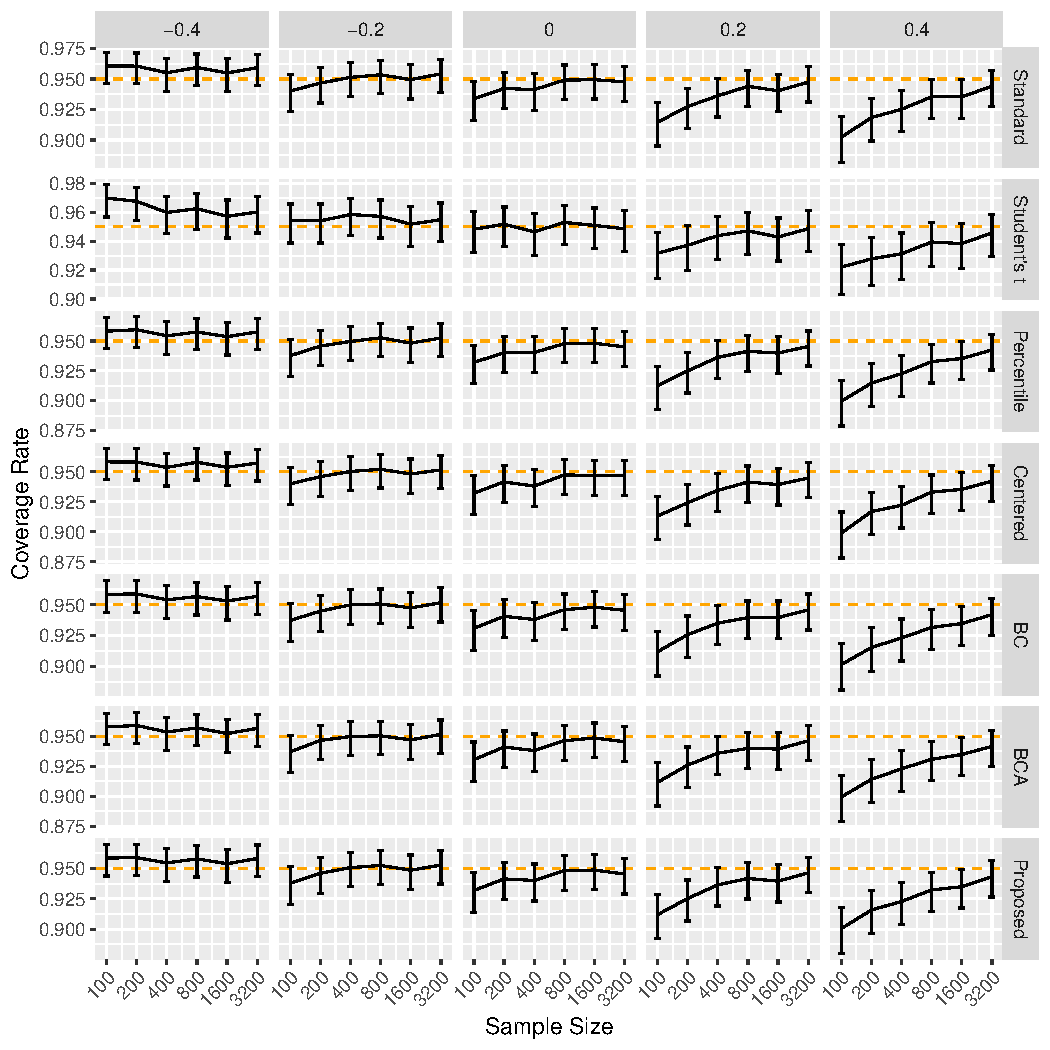
\includegraphics[width=\textwidth]{figures/plot_norm_mu}
  \caption{Empirical coverage rates of different 95\% block bootstrap CIs for
    the marginal mean $\mu$ of an AR(1) process with AR coefficient
    $\phi \in \{-0.4, 0.2, 0, 0.2, 0.4\}$ and series length
    $n \in \{100, 200, 400, 800, 1600, 3200\}$ based on 10,000 replicates. The
    error bars represent 95\% CIs of the real coverage rates.}
  \label{fig:mu}
\end{figure}


\begin{figure}[tbp]
  \centering
  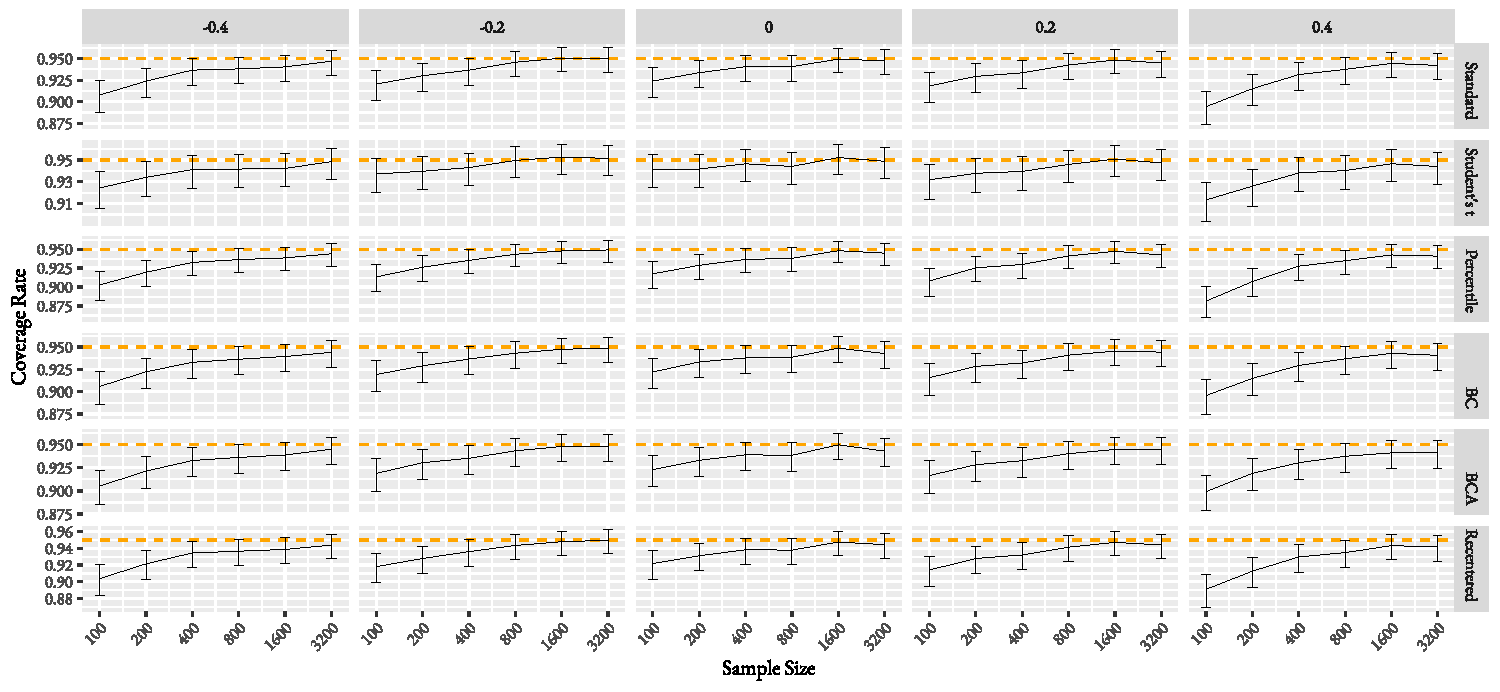
\includegraphics[width=\textwidth]{figures/plot_norm_sigma}
  \caption{Empirical coverage rates of different 95\% block bootstrap CIs for
    the marginal standard deviation $\sigma_x$ of an AR(1) 
    process with AR coefficient $\phi \in \{-0.4, 0.2, 0, 0.2, 0.4\}$ and
    series length $n \in \{100, 200, 400, 800, 1600, 3200\}$ based on 10,000
    replicates. The error bars represent 95\% CIs of the real coverage rates.}
  \label{fig:sigma}
\end{figure}


\begin{figure}[tbp]
  \centering
  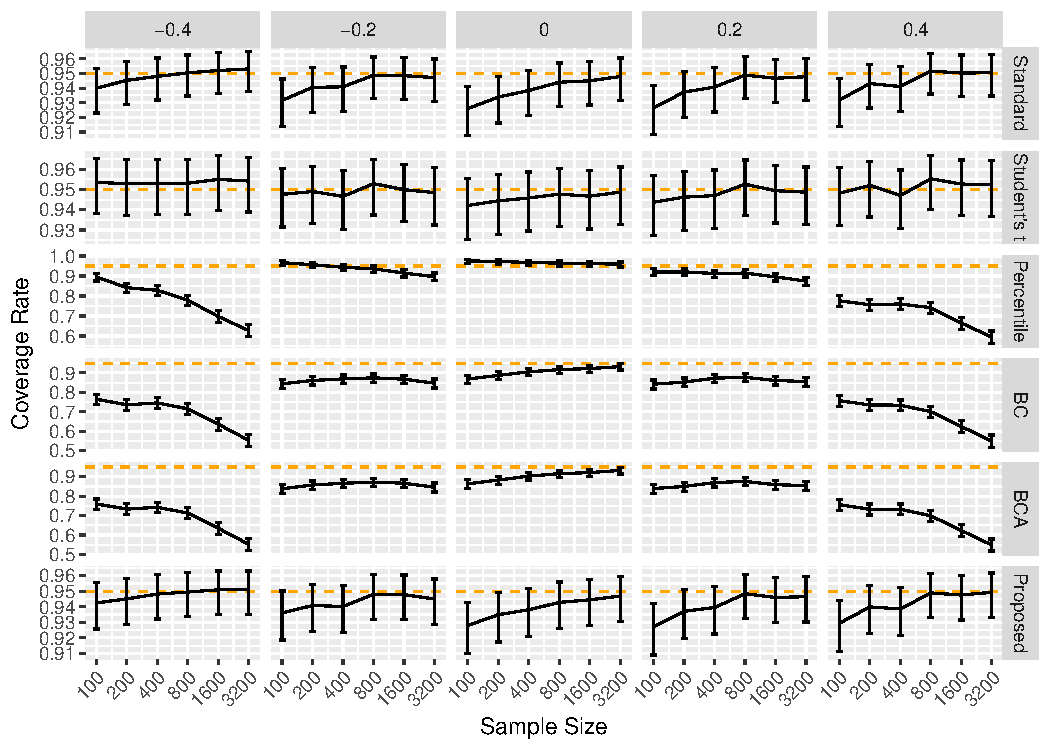
\includegraphics[width=\textwidth]{figures/plot_norm_phi}
  \caption{Empirical coverage rates of different 95\% block bootstrap CIs for
    the first-order autocorrelation coefficient $\phi$ of an AR(1) process with
    $\phi \in \{-0.4, 0.2, 0, 0.2, 0.4\}$ and series length
    $n \in \{100, 200, 400, 800, 1600, 3200\}$ based on 10,000 replicates. The
    error bars represent 95\% CIs of the real coverage rates.}
  \label{fig:phi}
\end{figure}


\subsection{Results}

For estimating the mean parameter~$\mu$, Figure~\ref{fig:mu} suggests that all
methods eventually approach correct coverage of $\mu$ as sample size
increases. Student's $t$ CIs appear to need the smallest sample size
to achieve correct coverage, except for samples with strong negative
dependence, in which case, they actually over-cover $\mu$ for smaller sample
sizes. For instance, for a sample with $n = 100$ and $\phi = -0.4$, the lower
bound for a Students $t$ CIs coverage of $\mu$ is greater than 95\%, whereas
the coverage intervals for other methods contain 95\%. The Standard,
Percentile, $BC$, and $BC_a$, and Recentered CIs require similar sample
sizes to recover $\mu$ at the nominal level for all combinations of $n$ and
$\phi$. All methods seem to require a smaller sample to recover $\mu$ at the
nominal rate when dealing with negative dependence versus positive dependence.
For example, $BC$ CIs recover $\mu$ for $n \geq 100$ when $\phi = -0.2$, but
they only recover $\mu$ for $n \geq 800$ when $\phi = 0.2$. In addition, as a
negative dependence gets stronger, holding everything else equal, coverage
increases, which lead to the Student $t$ CI's aforementioned over-coverage. As
a positive dependence gets stronger, holding everything else equal, coverage
decreases, and a larger sample is necessary to recover~$\mu$.


For estimating the standard deviation parameter~$\sigma_x$,
Figure~\ref{fig:sigma} suggests that every method can reach nominal coverage of
$\sigma_x$ if the sample is large enough, but for a given $n$ and $\phi$,
coverage of $\sigma_x$ will be lower than coverage of $\mu$ in general. Like
$\mu$, $\sigma_x$ can be covered by Student $t$ CIs with smaller sample sizes
when compared to other methods. Unlike $\mu$, there is no over-coverage issue for
$\sigma$ when $\phi = -0.4$. Standard, Percentile, $BC$, $BC_a$, and Recentered
CIs again have similar performance. All methods seem to have slightly higher
coverage of $\sigma_x$ when $\phi$ is negative versus when $\phi$ is positive.
Regardless of the sign, coverage of $\sigma_x$ gets worse as the strength of
the temporal dependence increases.
\jy{Compared to Figure 1, there is no over-coverage in this case. Say someting
  about this observation.} \mc{addressed}


For estimating the auto-correlation parameter~$\phi$, Figure~\ref{fig:phi}
suggests that while Standard, Student's $t$, and Recentered CIs do
approach correct coverage as sample size increases, Percentile, $BC$, and
$BC_a$ CIs deteriorate as sample size increases, especially as the strength of
the temporal dependence increases. Because of this, only Standard, Student's
$t$, and Recentered CIs should be considered as effective block bootstrap
methods to estimate $\phi$. Student's $t$ CIs once again can achieve correct
coverage with smaller sample sizes when compared to Standard and Recentered CIs
which perform similarly. Student's $t$ CIs can can recover $\phi$ at the
nominal level for $n \geq 100$ when the sample's temporal dependence is as
strong as 0.4. Coverage appears to be higher for all methods when the
dependence is negative rather than positive. Whether or not the dependence is
negative or positive, coverage of $\phi$ seems to increase slightly as the
absolute value increases for Standard, Student's $t$, and Recentereed CIs. For the
values of $\phi$ observed, there are no examples
of over-coverage for Standard, Student's $t$, $BC$, $BC_a$, or Recentered CIs.
However, Percentile CIs appear to over-cover $\phi$ for smaller sample sizes when 
$\phi = -0.2$ and when $\phi = 0$, indicating again that they should not be used.

\jy{Use cross for red. Otherwise, they are not distinguishable when printed in b/w.}
\mc{addressed}

\begin{figure}[tbp]
  \centering
  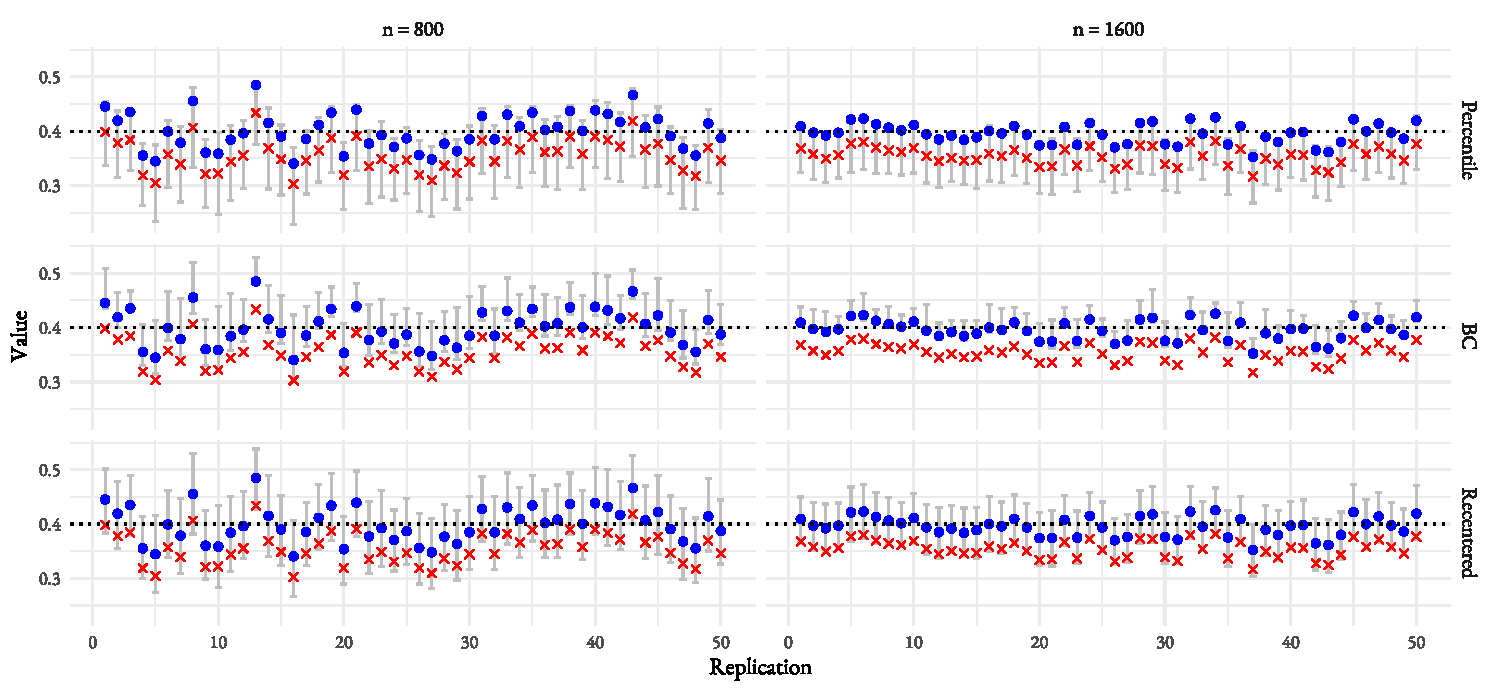
\includegraphics[width=\textwidth]{figures/norm_phi_intervals}
  \caption{100 replicate Percentile, Bias-Corrected, and Recentered
    Bootstrap CIs for samples of $n = 800$ for an AR(1) process with
    $\phi = 0.4$. For each replicate, the lower and upper bounds of the CIs
    are displayed, as well as $\hat\theta_n$ (blue circle) and
    $\bar\theta_n^{(b)}$ (red cross). }
  \label{fig:npi}
\end{figure}

\jy{can you also do the same plot for sample size 1600? And then put the two
  plots in one figure?} \mc{addressed}

The outcomes of the $\phi$ estimation raise a natural question about the
lackluster performance of certain methodologies. To delve into this inquiry, a
set of 100 CIs was generated for each of the percentile,
$BC$, and Recentered techniques. Illustrated in Figure~\ref{fig:npi}, it becomes
evident that the percentile-based CIs exhibit a notable bias, predominantly
manifesting as a substantial underestimation of $\phi$. On the other hand, $BC$
CIs do display a tendency to rectify this bias on average, albeit accompanied by
a rather inconsistent width across the intervals. Our Recentered CIs manage to
effectively mitigate the bias, employing $\widehat{\text{bias}} =
\bar\theta_n^{(b)} - \hat\theta_n$ as a corrective measure. Notably, this
correction often takes a negative form, indicative of a positive adjustment
arising from the interval construction detailed in Section~\ref{sec:bbci}.


To summarize, the performance of the CIs depends on the target parameter. When
estimating $\mu$ and $\sigma_x$, any CI will do, although Student's $t$ CIs
perform noticeably better than the others. However, when estimating $\phi$,
the choice of method is of utmost importance as to avoid coverage
deterioration. A smaller sample size is generally required to estimate a
parameter for a sample with a negative $\phi$ versus a positive $\phi$ of the
same magnitude. In order to know if coverage will increase as the strength of
the temporal dependence increases, one need to know what the parameter of
interest is, and in the case of $\mu$, the direction of the serial dependence. The
$BC$ approach does not seem to be correcting bias appropriately when estimating
$\phi$. Like the Percentile method, the Recentered method uses the spread from the 
bootstrap to construct the width of the CI. However, the Recentered approach, does
not correct from the original point estimate $\hat\theta_n$.
\jy{The BC approach appears not correcting the bias correctly. The Recentered
  approach simply does not correct point estimate and only uses the spreadness
  from the bootstrap to construct CIs.} \mc{addressed}


\section{Discussion}
\label{sec:disc}

Block bootstrap is a useful method for estimating parameters of a time series,
from simple parameters like the mean to more complicated temporal dependence
factors. We know theoretically that the block bootstrap procedure will cover
parameter of a time series at the nominal level given an infinitely large
sample, so the goal for this study was to find the smallest finite sample
length $n$ of a time series in order for the block bootstrap procedure to 
recover its associated parameters at an acceptable rate.
Our analysis relies on the assumption that there is a size $n$ large
enough for the method to work: that is, the method's performance improves as
$n$ increases. Out of the five types of intervals used in this study, this
assumption was found to hold true with respect to estimating $\phi$ only for
Standard, Student's $t$, and Recentered Method CIs, whereas Percentile, $BC$,
and $BC_a$ intervals exhibited coverage deterioration as $n$ increased. The
Percentile CI's coverage deterioration can be attributed to bias that is not
corrected as $n$ increases. Specifically, as $n$ increases, the width of the
CI decreases, but because the percentile CI underestimates $\phi$, the
coverage decreases. The $BC$ CI seems to correct the bias, but the width of
the CI seems to be inconsistent. The acceleration factor of the $BC_a$ CI
seems to fail, as the width of the CI seems to be inconsistent. 


\jy{use a better topic sentence.} \mc{addressed}
One of the goals of this study was to provide some practical recommendations for 
necessary sample sizes when using block bootstrap to estimate parameters of 
serially dependent data. When using Student's $t$ intervals and $\phi$ is unknown,
the results of this study suggest that an $n \geq 800$ may be necessary for common practice to
estimate simpler parameters like $\mu$ or $\sigma_x$. If $\phi$ is already
known, a lesser $n$ may be adequate to estimate these parameters. For lower
absolute values of $\phi$, a smaller $n$ is sufficient when estimating $\mu$
or $\sigma$. For negative values of $\phi$, coverage of $\mu$ is higher in
general. In fact, Student's $t$ seems to over-cover $\mu$ for $\phi = - 0.4$
when using smaller sample sizes, meaning that if $\phi$ is known to have a
very negative value, another CI may be required. However, in real world
applications, $\phi$ is more commonly found to be positive, so Student's $t$
should still be used if $\phi$ is unknown. Lastly, to estimate $\phi$,
$n \geq 100$ using the Student's $t$ method may be sufficient. Further
investigation may be necessary to see if there are other interval corrections
that fix the coverage deterioration problem for $\phi$.


This study could be used as a guide for applied statistics courses for students
to generally understand how large of a sample size is sufficient for block
bootstrap to be used versus other inference methods. For undergraduate or
graduate students, block bootstrap is not typically a part of curriculum, but
the results of this study can easily be used to demonstrate when it is
practical to use this method. This information could also prove to be useful
for research using block bootstrap estimation of time series in domains such
as econometrics. Future studies could investigate the $n$ needed to make
inferences about other forms
of serially dependent data such as a moving average process. One could also
investigate if there are types of block
bootstrap interval construction such as $ABC$ or bootstrap-t intervals, or
alternatives to block bootstrap, such as AR-Sieve bootstrap
 \citep{kreiss1992bootstrap}, that could more
\jy{Cite references for AR-sieve} \mc{addressed}
appropriately recover the parameters of a time series. In addition, as noted by
\citet{buhlmann2002bootstraps}, there are some 
general drawbacks of block bootstrap - with respect to how reasonably it imitates 
the data-generating process - which may be addressed in a future study.


\eds{Check out this paper:
Peter Buhlmann. "Bootstraps for Time Series." Statist. Sci. 17(1) 52 - 72, 
May 2002 - the conclusions of this paper are interesting in their own right:
``Disadvantages of the [block bootstrap] method include the following.
The block bootstrap sample should not be viewed as
a reasonable sample mimicking the data-generating
process: it is not stationary and exhibits artifacts where
resampled blocks are linked together. This implies that
the plug-in rule for bootstrapping an estimator $\hat{\theta}$ is not
appropriate. A prevectorization of the data is highly
recommended, but the bootstrapped estimator and its
computing routine may then need to be redesigned. As
a general nonparametric scheme, the block bootstrap
may be outperformed in various niches of stationary
time series, for example, for linear time series (see Section 3) 
and for categorical processes (see Section 5).
Second-order accuracy for a confidence interval has
been justified with the approach of Studentizing and
BCa correction (in the case of noncategorical time series); 
the latter was found to yield marginal improvement in a 
simulated example (we did not consider the former). } \mc{addressed}
	



\bibliographystyle{chicago}
\bibliography{citations}

\end{document}
